\section{Evaluation}
\label{sec:eval}
\paragraph{Setup.} All experiments run on the MacBook Air of Table~\ref{tab:model} with other applications closed. For the main decode experiments, all compared settings run interleaved in one process, so that they see the same cache state and the same background load. Each block decodes six tokens with one setting, the order of settings rotates every round, and we use three prompts in English and Chinese. We report the mean over blocks of the median time per token, with 95\% confidence intervals from Student's $t$ distribution, and we compare every block with the block of the reference setting from the same round. The evaluation answers three questions: how fast the system is, which kinds of parallelism help, and how close its output is to DeepSeek's own deployment.

\subsection{Speed and the cost model}
\label{sec:e2e}
Table~\ref{tab:results} summarizes the end-to-end results. With an expert cache that still leaves 9\,GB to macOS, \method{} decodes 1.23 tokens per second. Figure~\ref{fig:sweep} shows how decode speed depends on the size of the cache. Speed rises steadily as the cache grows, because every additional hit removes a read from the chain. Idle-window speculation shifts the whole curve upward. It is faster at every cache size, in 43 of 45 paired blocks, and it cuts the time spent waiting for the SSD by roughly a quarter.

\begin{table}[t]
\centering
\small
\caption{End-to-end results on a MacBook Air with 24\,GB. Decode uses idle-window speculation unless noted. Quality numbers come from teacher forcing against continuations sampled from DeepSeek's API.}
\label{tab:results}
\begin{tabular}{@{}lr@{}}
\toprule
Decode, 5.5\,GB expert cache, 9\,GB left to macOS & 1.23 tokens/s \\
Decode, 5.5\,GB expert cache, without speculation & 1.08 tokens/s \\
Decode, 6.5\,GB expert cache & 1.35 tokens/s \\
Speed-up from speculation, 2.5 to 6.5\,GB caches & 11--27\% \\
First token for a 14-token, 1K-token and 16K-token prompt & 10\,s, 49\,s, 9\,min \\
SSD read bandwidth with one or several reads in flight & 2.7, 3.0\,GB/s \\
Top-1 agreement on 129 open-ended continuation tokens & 86.0\% \\
Mean top-1 agreement over all 17 cases & 96.7\% \\
Mean NLL per token, ours and DeepSeek's API & 0.127, 0.046 \\
Needle retrieval, 12 lengths up to 16,385 tokens & 12 of 12 correct \\
\bottomrule
\end{tabular}
\end{table}

The cost model of Equation~\eqref{eq:chain} describes the runs without speculation closely. A two-parameter fit to the bytes each token has to read matches all five cache sizes within two percent. Applied to the runs with speculation, the same fit predicts that they should be even faster than they are, because it ignores the speculative reads. Those reads are not free: about half of their volume still costs time, and the other half falls into time when the SSD would have been idle. The traces confirm this directly. Without speculation the SSD is busy for less than two thirds of a decode step, and with speculation the busy share rises by roughly a fifth, almost all of it taken up by reads that overlap no demand read.

\begin{figure}[t]
\centering
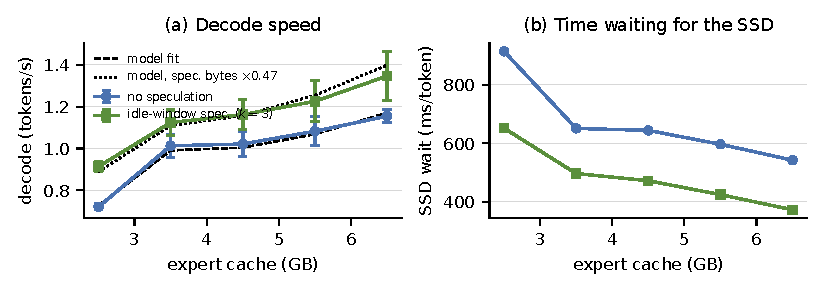
\includegraphics[width=0.9\linewidth]{figures/sweep.pdf}
\caption{(a) Decode speed against expert cache size, with and without idle-window speculation, interleaved in one process with 95\% confidence intervals over nine blocks. The dashed line is the cost model $t=C+D/B$ fitted to the runs without speculation, with $C=117$\,ms and $B=2.37$\,GB/s, which matches them within 2\%. The dotted line adds the speculative bytes with weight $\alpha=0.47$, fitted on the same runs. (b) Time per token spent waiting for the SSD.}
\label{fig:sweep}
\end{figure}

\paragraph{Prefill.} Prefill behaves differently from decode. Even a short prompt routes to most experts of every layer, so the first chunk reads nearly the whole expert set once, and long prompts are limited by GPU compute rather than by the SSD. Bounded replay keeps the later layers out of most of that work. We prefill in chunks of 4K tokens, because a single long chunk is no faster and needs considerably more memory at its peak.

\subsection{Where does parallelism help?}
\label{sec:parallel-eval}
We now return to the question of the introduction and look at each level of the system where parallelism could help. Table~\ref{tab:ablation} and Figure~\ref{fig:parallel} show the interleaved ablation of the decode schedule, and Table~\ref{tab:negative} collects the other techniques we tried.

\begin{table}[t]
\centering
\small
\caption{Decode schedules at a 5\,GB cache, interleaved in one process. Speed-ups are paired against the serial schedule of the same round, with 95\% confidence intervals over 12 blocks. All speculative schedules read three guesses per layer. In the first run the naive prefetcher ranks its guesses by the raw gate logits; the second run repeats the key schedules with the router's exact scoring for every prefetcher. Tokens per second and SSD wait are from the first run.}
\label{tab:ablation}
\resizebox{\linewidth}{!}{%
\begin{tabular}{@{}lccrrrr@{}}
\toprule
Schedule & Guesses wait & Guesses cold & Tokens/s & SSD wait, ms & Speed-up, run 1 & Speed-up, run 2 \\
\midrule
Serial & & & 1.03 & 630 & 1.00 & 1.00 \\
Overlap cached and missing experts & & & 1.07 & 617 & $1.05\pm0.04$ & \\
Naive next-layer prefetch \citep{moeoffload} & no & no & 0.97 & 667 & $0.95\pm0.07$ & $0.89\pm0.05$ \\
Guesses issued with the demand reads & no & no & 0.99 & 637 & $0.96\pm0.05$ & \\
Guesses inserted cold only & no & yes & 0.87 & 770 & $0.85\pm0.06$ & \\
Guesses wait for demand reads only & yes & no & 1.17 & 464 & $1.15\pm0.05$ & $1.10\pm0.05$ \\
\textbf{Idle-window speculation} & yes & yes & \textbf{1.20} & \textbf{456} & $\mathbf{1.17\pm0.05}$ & $\mathbf{1.14\pm0.05}$ \\
\bottomrule
\end{tabular}}
\end{table}

\begin{figure}[t]
\centering
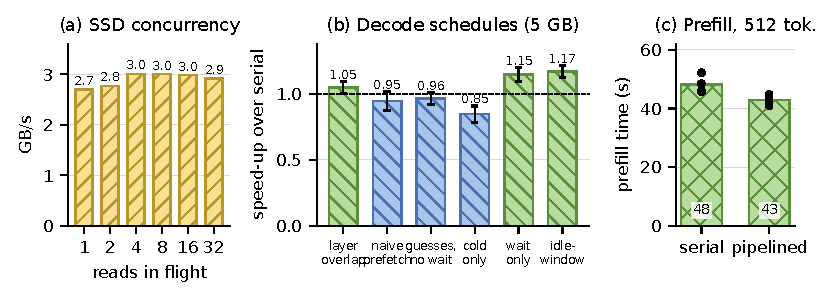
\includegraphics[width=\linewidth]{figures/parallel.pdf}
\caption{Parallelism on one laptop. (a) Read bandwidth for expert records against the number of reads in flight. (b) The first run of the schedule ablation in Table~\ref{tab:ablation}, as speed-up over the serial schedule with 95\% confidence intervals; green marks schedules that are faster than serial. (c) Prefill of a 512-token prompt with and without reading the next batch of experts while the current one computes; bars show means and dots individual runs.}
\label{fig:parallel}
\end{figure}

\paragraph{Inside the SSD.} The drive itself is the one place where parallelism comes for free. It delivers expert records noticeably faster with several requests in flight than with one, and it saturates after a few, which our eight I/O threads easily provide. Splitting a single expert into smaller reads adds nothing, because a read of an entire expert is already large.

\paragraph{Inside a layer.} Computing the cached experts while the missing ones load is the closest match to the cluster's micro-batch overlap. It helps a little. Figure~\ref{fig:timeline}a shows why it cannot help more: the cached experts of a layer take a few milliseconds to compute, while the reads take several times longer.

\paragraph{Across layers.} This is where the schedule matters most. Naive prefetching of the next layer's experts is slower than not prefetching at all, in both runs of the ablation. It even collects twice as many speculative hits as idle-window speculation and still loses, because its guesses compete with the reads the token is waiting for. Making the guesses wait for those reads is what turns the loss into a gain, and it accounts for almost all of the improvement. Inserting the guesses cold adds a little on top, within the confidence interval. On its own, cold insertion is harmful, because guesses that arrive too early are evicted again before the next layer can use them. With both changes, idle-window speculation was faster than the serial schedule in 23 of 24 paired blocks across the two runs, and it produced exactly the same tokens as decoding without it. Three guesses per layer worked best; with more, the guesses again started to delay demand reads.

\paragraph{Across expert batches in prefill.} During prefill a whole chunk of tokens goes through each layer, which gives the engine something like a batch. Reading the next batch of experts while the current one computes made prefill about a tenth faster on an otherwise idle machine. In an earlier session with other programs holding memory, the same pipelining caused swapping and gained nothing, because the extra batch needs room.

\paragraph{Across tokens.} Speculative decoding checks several drafted tokens in one pass \citep{specdecoding}. On a GPU this amortizes weight reads over several tokens. Here the drafted tokens route to different experts, so the check must read the union of their experts, and decode became several times slower. The controller described in Section~\ref{sec:impl} detects this and falls back to plain decoding.

\paragraph{In the operating system.} The page cache could in principle serve as a larger second-level cache behind the slab. In practice it competes with the slab for the same memory, and no setting we tried was faster than bypassing it.

\begin{table}[t]
\centering
\small
\caption{Other techniques, each measured against a baseline from the same session in tokens per second, or in seconds for prefill.}
\label{tab:negative}
\resizebox{\linewidth}{!}{%
\begin{tabular}{@{}p{0.42\linewidth}rrp{0.28\linewidth}@{}}
\toprule
Technique & Without & With & Note \\
\midrule
Pipelined expert batches in prefill, 512 tokens & 48.1\,s & 42.8\,s & interleaved, four runs each \\
Four-way split reads per expert & 1.12 & 1.11 & \\
OS page cache behind a 5\,GB slab & 1.12 & 0.20--0.61 & \\
DSpark speculative decoding, fixed draft length & 1.28 & 0.35 & \\
Two, three, four or six guesses per layer & & 1.13, 1.19, 1.14, 1.06 & same day, not interleaved \\
\bottomrule
\end{tabular}}
\end{table}

Taken together, the measurements give a simple rule. Parallelism pays off when it gives the SSD work during time that the dependency chain would leave idle, without delaying a read the token is waiting for and without taking memory from the cache. Idle-window speculation meets all three conditions, while naive prefetching, speculative decoding and the page cache each break one of them. Even so, the size of the cache remains the strongest single factor.

\subsection{Output quality}
\label{sec:quality}
We compare \method{} with DeepSeek's own deployment using continuations sampled from DeepSeek's API, published with the ds4 project \citep{ds4}, and run them through the converted model with teacher forcing. Figure~\ref{fig:api} shows top-1 agreement for each case. On the five open-ended continuations, our model picks the same next token as the API for 86\% of the tokens. The gap comes from compressing the experts to two or three bits, which matters more for free text than for retrieval. The other twelve cases are needle-retrieval prompts whose lengths sit just around the sliding window, the boundaries of the key selection and the candidate-block level. The model answers all of them correctly, which shows that the long-context machinery works as in the reference.

\begin{figure}[t]
\centering
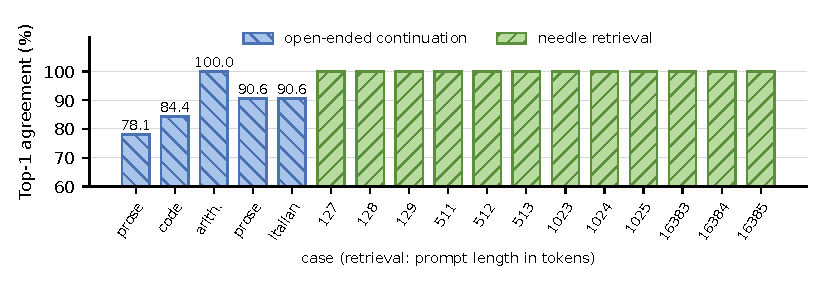
\includegraphics[width=0.9\linewidth]{figures/api_cases.pdf}
\caption{Top-1 agreement with continuations sampled from the official API. The retrieval prompts have one-token answers.}
\label{fig:api}
\end{figure}
